\documentclass{article}
\usepackage[utf8]{inputenc}
\usepackage{geometry}
\usepackage{subcaption} %Sub figures
 \geometry{
 a4paper,
 total={170mm,257mm},
 left=20mm,
 top=20mm,
 }
 \usepackage{graphicx}
 \usepackage{titling}

 \newcommand\tab[1][1cm]{\hspace*{#1}}

 \title{Developing a Task Allocator Using Network Flow and Linear Programming}
\author{Stella Rovazzi}
\date{Summer 2025}
 
 \usepackage{fancyhdr}
\fancypagestyle{plain}{%  the preset of fancyhdr 
    \fancyhf{} % clear all header and footer fields
    \fancyfoot[L]{\thedate}
    \fancyhead[L]{Task Allocator}
    \fancyhead[R]{\theauthor}
}
\makeatletter
\def\@maketitle{%
  \newpage
  \null
  \vskip 1em%
  \begin{center}%
  \let \footnote \thanks
    {\LARGE \@title \par}%
    \vskip 1em%
    %{\large \@date}%
  \end{center}%
  \par
  \vskip 1em}
\makeatother

\usepackage{lipsum}  
\usepackage{cmbright}

\begin{document}

\maketitle

\section*{Project Goal}
\tab The goal of this project is to develop a program that helps a group of people allocate tasks based on individuals' willingness to perform certain tasks and 
the importance of the task. I aim to apply this to two situations. The first is a house cleaning scenario, where roommates are able to divide up their weekly chores based on preference, ensuring
that everything is completed at least every two weeks. The second is inspired by my robotics team and sets up a more complex scenario involving more conditionals. This new task allocator must divide
tasks based on preference, skill, number of people per certain task, and time available. The first scenario, should solely be able to use a maximum flow algorithms. However, the extra constraints
 in the second scenario make it more easily solved with linear programming approach.

\section*{Scenario One - House Chores}
\subsection*{Laying out the Problem}
\tab This problem can be represented as a network graph, shown in \textit{Figure 1a}. This will allow us to use a maximum-flow algorithm to divide up the tasks. To ensure that I can use a network flow algorithm, I've added in
total sources and sinks, shown in \textit{Figure 1b}.
\begin{figure}[ht!]
  \subcaptionbox*{A: Original Graph}[.3\linewidth]{
    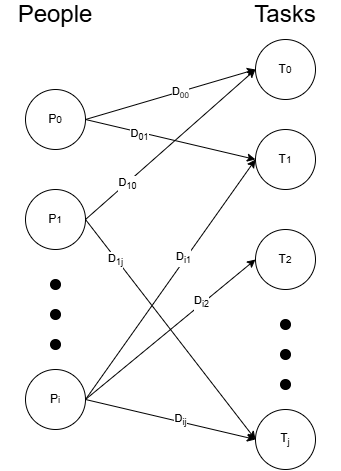
\includegraphics[width=\linewidth]{fig1.png}
  }
  \hfill
  \subcaptionbox*{B: With Source and Sink}[.55\linewidth]{
    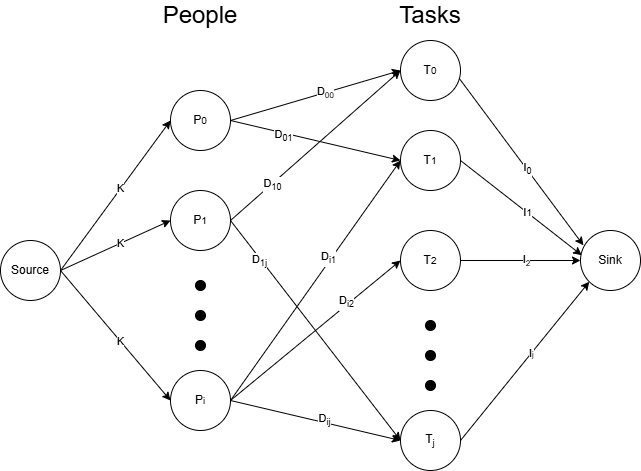
\includegraphics[width=\linewidth]{fig1b.png}
  }

  \caption{Graph Network of Hosue Chore Scenario}
In these diagrams, the notation is as follows: \\
\tab People are represented by $P_0, P_1, ..., P_i$ \\
\tab Tasks are represented by $T_0, T_1, ..., T_j$ \\
\tab The desires of a specific person to do a certain task are represented by $D_{00}, D_{01}, ..., D_{ij}$ \\
\tab The importance of a specific tasks is represented by $I_0, I_1, ..., I_j$ \\
\tab $K$ represents the maximum number of tasks each person is allowed to be assigned.
\end{figure}

\section*{Scenario Two - Robotics Tasks}



\end{document}